

\section{État de l'art}
\label{repl:sec:stateoftheart}

Dès 1975, les bases de données répliquées font leur
apparition~\cite{johnson1975maintenance} afin de résoudre
\begin{inparaenum}[(i)]
\item les problèmes de défaillances~\cite{alsberg1976principle}, i.e., le
  serveur possédant les données étant inaccessible, le client peut contacter
  serveur alternatif connu pour posséder les mêmes données afin de satisfaire sa
  requête;
\item les problèmes de rapidité d'accès, i.e., le client peut contacter un
  serveur avec lequel la latence est faible afin de satisfaire plus rapidement
  sa requête.
\end{inparaenum}

Cependant la réplication introduit un nouveau type de problèmes : la
synchronisation des répliques. En effet, puisque la communication entre serveurs
n'est pas instantanée, les modifications effectuées sur les données prennent du
temps à parvenir aux répliques. Cela implique des problèmes de
\begin{inparaenum}[(i)]
\item fraîcheur de données -- \emph{est-ce que la donnée que j'obtiens est la
    plus à jour ?} -- et de
\item modifications concurrentes -- \emph{avec des modifications effectuées sur
    une même données, au même moment, par deux serveurs distants dont les
    résultats sont différents. Dois-je conserver les deux modifications, ou
    dois-je en privilégier une, ou dois-je employer une autre stratégie ?}
\end{inparaenum}


D'après le théorème CAP~\cite{brewer2012cap, gilbert2002brewer} il est
impossible de répliquer sur un grand nombre de serveurs tout en garantissant la
cohérence forte~\cite{herlihy1990linearizability}, la disponibilité, et la
tolérances aux partitionnements. Dans ce manuscrit, nous nous intéressons aux
applications garantissant ces deux dernières propriétés. Ainsi, une opération
est toujours acceptée par le système. De plus, le système, constitué de
plusieurs serveurs distants, autorise la fragmentation temporaire en
ilôts. Par conséquent, le critère de cohérence doit être
affaiblit~\cite{bailis2013eventual, shapiro2011conflict}.

Le reste de cette section décrit le schéma garantissant les deux propriétés
recherchées, à savoir la réplication optimiste (cf. §\ref{repl:subsec:optimistic}).
Ensuite, elle passe en revue deux familles d'approches appartenant à la
réplication optimiste : les transformées opérationnelles et les structures de
données répliquées sans résolution de conflits
(cf. §\ref{repl:subsec:otorcrdts}). Enfin, nous nous intéresserons plus
particulièrement aux types de données représentant les séquences -- la séquence
de caractères étant proche d'un document (cf. §\ref{repl:subsec:sequences}). 

% \subsection{Pessimisme ou optimisme ?}
% \label{repl:subsec:schemas}

% De multiples serveurs, possiblement distants les uns des autres, hébergent une
% réplique d'une donnée. Lorsqu'une réplique est modifiée, sa modification est
% répercutée sur les autres répliques. Les deux schémas de réplication définissent
% la manière dont une modification est acceptée. Cela influe sur les propriétés du
% système. En particulier, les dimensions que peuvent atteindre les systèmes, en
% nombre de répliques, s'en trouve impactées.

% \subsubsection{Réplication pessimiste}
% \label{repl:subsubsec:pessimistic}

% L'objectif de la réplication pessimiste est simple. Il consiste à donner
% l'illusion que la donnée manipulée est unique, indépendemment du nombre de
% répliques réel. Ainsi, il devient facile de raisonner sur les données puisque
% leurs spécifications sont proches de celles proposées dans un contexte sans
% réplications.  Toutefois, avant qu'une modification ne soit réellement
% effectuée, il est nécessaire qu'elle soit validée. L'autorité décisionnelle
% diffère en fonction des approches :

% \paragraph{Autorité centrale~\cite{alsberg1976principle} :} Un serveur est
% désigné responsable. Ceux qui souhaitent modifier la donnée sont alors dans
% l'obligation de demander l'accès exclusif pendant la mise en place de cette
% modification. Dans l'intervalle, les autres répliques ne peuvent soumettre de
% modifications. Enfin, lorsque la modification est achevée, la main est rendue au
% serveur qui peut autoriser d'autres modifications. On parle de verrou
% (\emph{lock}).

% \paragraph{Quorum~\cite{gifford1979weighted} :} Un ensemble de serveurs est
% désigné responsable. Chacune des modifications est soumise à un vote quant à son
% acceptation. Au dessus d'un certain seuil de vote positif ou négatif, la
% modification est autorisée ou non.



% \begin{figure*}
%   \centering
%   \subfloat[Une demande de modification est effectuée]
%   [Le serveur $n_5$ demande au cœur décisionnel si sa modification est acceptée.]
%   {
\begin{tikzpicture}[scale=1.2]

  \newcommand\X{35pt};
  \newcommand\Y{35pt};

  \draw[fill=white, very thick](0*\X, 0*\Y)
  node{$n_1$} +(-5pt,-5pt) rectangle +(5pt,5pt);
  \draw[fill=white, very thick](1*\X,-1*\Y)
  node{$n_2$} +(-5pt,-5pt) rectangle +(5pt,5pt);
  \draw[fill=white, very thick](2*\X, 0*\Y)
  node{$n_3$} +(-5pt,-5pt) rectangle +(5pt,5pt);

  \draw[fill=white](-1.5*\X,0*\Y) node{$n_4$} +(-5pt,-5pt) rectangle +(5pt,5pt);
  \draw[fill=white, thick, draw=darkblue](-1.5*\X,1*\Y)
  node{\DARKBLUE{$n_5$}} +(-5pt,-5pt) rectangle +(5pt,5pt);
  
  \draw[<->] (5+0*\X, 0*\Y) -- (-5+2*\X,0*\Y);
  \draw[<->] (0*\X, -5+0*\Y) -- (-5+1*\X,-1*\Y);
  \draw[<->] (2*\X, -5+0*\Y) -- (5+1*\X ,-1*\Y);

  \scriptsize
  \draw[<->] (5-1.5*\X,0*\Y) -- (-5+0*\X,0*\Y);
  \draw[->, thick, draw=darkblue] (5-1.5*\X, 1*\Y) --
  node[anchor=south west, align=left]
  {\DARKBLUE{ask permission}\\\DARKBLUE{for modification}\\\DARKBLUE{on replica}}
  (-5+0*\X,5+0*\Y);
  
  \draw(1*\X, -0.5*\Y) node[anchor=south, align=center]{decisionnal\\chamber};

  % \scriptsize
  % \draw[->,dashed,very thick, color=darkblue](5+0*\X, 0*\Y) -- 
  % node[anchor=south]{(a)}(-5+ 2*\X, 0*\Y);
  % \draw[->] (-5+2*\X, 5pt) -- (5+\X, \Y);
  % \draw[->] (-5+2*\X, 5pt) --  (5+\X, 2*\Y);
  % \draw[->] (-5+2*\X, -5pt) -- (5+\X, -\Y);
  % \draw[->] (-5+2*\X, -5pt) -- (5+\X, -2*\Y);

  % \normalsize
  % \draw[fill=white, very thick, draw=darkblue]
  % (0*\X, 0*\Y) node{\DARKBLUE{$n_1$}} +(-5pt,-5pt) rectangle +(5pt,5pt);
  % \draw[fill=white, very thick]
  % (2*\X, 0*\Y) node{$n_2$} +(-5pt,-5pt) rectangle +(5pt,5pt);

  % \draw[fill=white](1*\X,2*\Y) node{$n_6$} +(-5pt,-5pt) rectangle +(5pt,5pt);
  % \draw[fill=white](1*\X,1*\Y) node{$n_5$} +(-5pt,-5pt) rectangle +(5pt,5pt);
  % \draw[fill=white](1*\X,-1*\Y) node{$n_4$} +(-5pt,-5pt) rectangle +(5pt,5pt);
  % \draw[fill=white](1*\X,-2*\Y) node{$n_3$} +(-5pt,-5pt) rectangle +(5pt,5pt);
  
\end{tikzpicture}}
%   \hspace{40pt}
%   \subfloat[Une autre demande est faite pendant que le cœur s'occupe de 
%   la première demande]
%   [Le serveur $n_4$ demande également si sa modification est acceptée pendant
%   que le cœur est occupé avec la modification de $n_5$.]
%   {
\begin{tikzpicture}[scale=1.2]

  \newcommand\X{35pt};
  \newcommand\Y{35pt};

  \draw[fill=white, very thick](0*\X, 0*\Y)
  node{$n_1$} +(-5pt,-5pt) rectangle +(5pt,5pt);
  \draw[fill=white, very thick](1*\X,-1*\Y)
  node{$n_2$} +(-5pt,-5pt) rectangle +(5pt,5pt);
  \draw[fill=white, very thick](2*\X, 0*\Y)
  node{$n_3$} +(-5pt,-5pt) rectangle +(5pt,5pt);

  \draw[fill=white, thick, draw=darkblue](-1.5*\X,0*\Y)
  node{\DARKBLUE{$n_4$}} +(-5pt,-5pt) rectangle +(5pt,5pt);
  \draw[fill=white](-1.5*\X,1*\Y) node{$n_5$} +(-5pt,-5pt) rectangle +(5pt,5pt);

  \scriptsize  
  \draw[<-, thick, draw=darkblue] (5+0*\X, 0*\Y) --
  node[anchor=south]{\DARKBLUE{Ok. Ok?}} (-5+2*\X,0*\Y);
  \draw[->, thick, draw=darkblue] (0*\X, -5+0*\Y) --
  node[anchor=east]{\DARKBLUE{Ok. Ok?}}  (-5+1*\X,-1*\Y);
  \draw[<-, thick, draw=darkblue] (2*\X, -5+0*\Y) --
  node[anchor=west]{\DARKBLUE{Ok. Ok?}} (5+1*\X ,-1*\Y);


  \draw[->, draw=darkblue] (5-1.5*\X,0*\Y) --
  node[anchor=north]{\DARKBLUE{ask permission}}
  (-5+0*\X,0*\Y);
  \draw[<->] (5-1.5*\X, 1*\Y) -- node[anchor=south west]{wait}
  (-5+0*\X,5+0*\Y);
  
  \draw(1*\X, -0.5*\Y) node[anchor=south, align=center]{decisionnal\\chamber};

  % \scriptsize
  % \draw[->,dashed,very thick, color=darkblue](5+0*\X, 0*\Y) -- 
  % node[anchor=south]{(a)}(-5+ 2*\X, 0*\Y);
  % \draw[->] (-5+2*\X, 5pt) -- (5+\X, \Y);
  % \draw[->] (-5+2*\X, 5pt) --  (5+\X, 2*\Y);
  % \draw[->] (-5+2*\X, -5pt) -- (5+\X, -\Y);
  % \draw[->] (-5+2*\X, -5pt) -- (5+\X, -2*\Y);

  % \normalsize
  % \draw[fill=white, very thick, draw=darkblue]
  % (0*\X, 0*\Y) node{\DARKBLUE{$n_1$}} +(-5pt,-5pt) rectangle +(5pt,5pt);
  % \draw[fill=white, very thick]
  % (2*\X, 0*\Y) node{$n_2$} +(-5pt,-5pt) rectangle +(5pt,5pt);

  % \draw[fill=white](1*\X,2*\Y) node{$n_6$} +(-5pt,-5pt) rectangle +(5pt,5pt);
  % \draw[fill=white](1*\X,1*\Y) node{$n_5$} +(-5pt,-5pt) rectangle +(5pt,5pt);
  % \draw[fill=white](1*\X,-1*\Y) node{$n_4$} +(-5pt,-5pt) rectangle +(5pt,5pt);
  % \draw[fill=white](1*\X,-2*\Y) node{$n_3$} +(-5pt,-5pt) rectangle +(5pt,5pt);
  
\end{tikzpicture}}
%   \hspace{10pt}
%   \subfloat[Une modification est acceptée pendant que l'autre est refusée]
%   [La modification de $n_5$ est acceptée tandis que celle de $n_4$ 
%   est refusée.]
%   {
\begin{tikzpicture}[scale=1.2]

  \newcommand\X{35pt};
  \newcommand\Y{35pt};

  \draw[fill=white, very thick](0*\X, 0*\Y)
  node{$n_1$} +(-5pt,-5pt) rectangle +(5pt,5pt);
  \draw[fill=white, very thick](1*\X,-1*\Y)
  node{$n_2$} +(-5pt,-5pt) rectangle +(5pt,5pt);
  \draw[fill=white, very thick](2*\X, 0*\Y)
  node{$n_3$} +(-5pt,-5pt) rectangle +(5pt,5pt);

  \draw[fill=white](-1.5*\X,0*\Y) node{$n_4$} +(-5pt,-5pt) rectangle +(5pt,5pt);
  \draw[fill=white](-1.5*\X,1*\Y)
  node{$n_5$} +(-5pt,-5pt) rectangle +(5pt,5pt);
  
  \draw[<->] (5+0*\X, 0*\Y) -- (-5+2*\X,0*\Y);
  \draw[<->] (0*\X, -5+0*\Y) -- (-5+1*\X,-1*\Y);
  \draw[<->] (2*\X, -5+0*\Y) -- (5+1*\X ,-1*\Y);

  \scriptsize
  \draw[<-, thick, draw=darkblue] (5-1.5*\X,0*\Y) --
  node[anchor=north]{\DARKBLUE{denied}}(-5+0*\X,0*\Y);
  \draw[<-, thick, draw=darkblue] (5-1.5*\X, 1*\Y) --
  node[anchor=south west]{\DARKBLUE{accepted}}(-5+0*\X,5+0*\Y);
  
  \draw(1*\X, -0.5*\Y) node[anchor=south, align=center]{decisionnal\\chamber};

  % \scriptsize
  % \draw[->,dashed,very thick, color=darkblue](5+0*\X, 0*\Y) -- 
  % node[anchor=south]{(a)}(-5+ 2*\X, 0*\Y);
  % \draw[->] (-5+2*\X, 5pt) -- (5+\X, \Y);
  % \draw[->] (-5+2*\X, 5pt) --  (5+\X, 2*\Y);
  % \draw[->] (-5+2*\X, -5pt) -- (5+\X, -\Y);
  % \draw[->] (-5+2*\X, -5pt) -- (5+\X, -2*\Y);

  % \normalsize
  % \draw[fill=white, very thick, draw=darkblue]
  % (0*\X, 0*\Y) node{\DARKBLUE{$n_1$}} +(-5pt,-5pt) rectangle +(5pt,5pt);
  % \draw[fill=white, very thick]
  % (2*\X, 0*\Y) node{$n_2$} +(-5pt,-5pt) rectangle +(5pt,5pt);

  % \draw[fill=white](1*\X,2*\Y) node{$n_6$} +(-5pt,-5pt) rectangle +(5pt,5pt);
  % \draw[fill=white](1*\X,1*\Y) node{$n_5$} +(-5pt,-5pt) rectangle +(5pt,5pt);
  % \draw[fill=white](1*\X,-1*\Y) node{$n_4$} +(-5pt,-5pt) rectangle +(5pt,5pt);
  % \draw[fill=white](1*\X,-2*\Y) node{$n_3$} +(-5pt,-5pt) rectangle +(5pt,5pt);
  
\end{tikzpicture}}
%   \caption[Quorum en réplication pessimiste]
%   {\label{repl:fig:pessimisticexample} Exemple de quorum en réplication
%     pessimiste. La modification de $n_5$ est propagée.}
% \end{figure*}

% La figure~\ref{repl:fig:pessimisticexample} montre un exemple de réplication
% pessimiste où le cœur décisionnel est composé de 3 serveurs
% $\{n_1,\, n_2,\, n_3\}$ devant unanimement approuver une modification avant
% qu'elle soit propagée. Ainsi, le serveur $n_5$ propose une modification des
% répliques au cœur décisionnel via $n_1$. Ce dernier l'accepte et transmet la
% demande à $n_2$, qui l'accepte et la transmet à son tour à $n_3$, qui l'accepte
% et termine la boucle en transmettant à $n_1$.  Dans l'intervalle, $n_4$ propose
% une autre modification. La proposition de $n_5$ est acceptée et propagée tandis
% que celle de $n_4$ est refusée. Une fois que $n_4$ a reçu les modifications de
% $n_5$, il peut retenter de transmettre sa modification s'il la juge toujours
% d'actualité. Cet exemple illustre le caractère chronophage du processus : le
% vote prend du temps et peut échouer. De plus, si l'un des serveurs du cœur
% défaillit, le vote peut échouer alors même que la modification est valide.

% La réplication pessimiste est possible lorsque le nombre de répliques est connu,
% plutôt petit, et souvent accessible. Ces contraintes sont notamment
% satisfaisable dans le Nuage~\cite{mell2011national}. Les répliques proposent
% d'avantage de garanties quant aux résultats de la manipulation des
% données. Toutefois, de telles garanties ne sont pas toujours nécessaires et
% leur coût élevé n'est plus justifié. La réplication optimiste constitue alors
% une alternative possible.

\subsection{Réplication optimiste de séquences}
\label{repl:subsec:optimistic}

% En 1987, Demers et al. décrivent une base de données répliquée sur plusieurs
% centaines de machines pouvant communiquer entre elles au travers de matériels
% aux capacités hétérogènes~\cite{demers1987epidemic}. Du fait de ces dimensions,
% la réplication pessimiste~\cite{alsberg1976principle, gifford1979weighted}, où
% les opérations doivent être approuvées avant d'être appliquées, semble
% impossible.

La réplication optimiste~\cite{demers1987epidemic, johnson1975maintenance,
  ladin1992providing, saito2005optimistic} est un paradigme de réplication
consistant à appliquer les modifications directement sur une réplique locale.
Ainsi, les données sont toujours disponibles et réactives aux changements
effectués. Ensuite, les modifications sont disséminées aux autres serveurs
hébergeant une réplique où elles sont appliquées. Au contraire des approches
pessimistes~\cite{alsberg1976principle, gifford1979weighted}, les approches
optimistes ne verrouillent pas les données lors des changements. En revanche, le
critère de cohérence assuré est plus faible. En particulier, l'état des
répliques peut être temporairement différent :


\paragraph{Cohérence à terme~\cite{bailis2013eventual} :} Lorsque toutes les
modifications ont été reçues et intégrées par toutes les répliques, celles-ci
possèdent un état équivalent.

\noindent Puisque ``\emph{toutes} les modifications'' constitue un ensemble peu
réaliste pour raisonner sur une exécution réelle, une définition plus précise
porte sur un sous-ensemble de ces modifications :

\paragraph{Cohérence forte à terme~\cite{shapiro2011conflict} :} Les répliques
ayant reçu et intégré les mêmes modifications possèdent un état équivalent.


\begin{figure*}
  \centering
  \subfloat[Modifications concurrentes]
  [Les serveurs $n_1$ et $n_3$ modifient leur couleur en même temps.]
  {
\begin{tikzpicture}[scale=1.2]

  \newcommand\X{35pt};
  \newcommand\Y{40pt};

  %% spacing
  \draw (1*\X, -2*\Y);

  \draw[fill=darkblue, very thick](0*\X, 0*\Y)
  node{$n_1$} +(-5pt,-5pt) rectangle +(5pt,5pt);
  \draw[fill=white, very thick](1*\X,-1*\Y)
  node{$n_2$} +(-5pt,-5pt) rectangle +(5pt,5pt);
  \draw[fill=white, very thick](2*\X, 0*\Y)
  node{$n_3$} +(-5pt,-5pt) rectangle +(5pt,5pt);

  \scriptsize
  \draw[<-] (5+0*\X, -3+0*\Y) --
  node[anchor=north]{change to white}(-5+2*\X, -3+0*\Y);
  \draw[->] (5+0*\X,  3+0*\Y) --
  node[anchor=south]{change to \DARKBLUE{blue}}(-5+2*\X, 3+0*\Y);

  \draw[->] (0*\X, -5+0*\Y) --
  node[anchor=north east]{change to \DARKBLUE{blue}} (-5+1*\X, -1*\Y);

  \draw[->] (2*\X, -5+0*\Y) --
  node[anchor=north west]{change to white} ( 5+1*\X, -1*\Y);

  % \scriptsize
  % \draw[->,dashed,very thick, color=darkblue](5+0*\X, 0*\Y) -- 
  % node[anchor=south]{(a)}(-5+ 2*\X, 0*\Y);
  % \draw[->] (-5+2*\X, 5pt) -- (5+\X, \Y);
  % \draw[->] (-5+2*\X, 5pt) --  (5+\X, 2*\Y);
  % \draw[->] (-5+2*\X, -5pt) -- (5+\X, -\Y);
  % \draw[->] (-5+2*\X, -5pt) -- (5+\X, -2*\Y);

  % \normalsize
  % \draw[fill=white, very thick, draw=darkblue]
  % (0*\X, 0*\Y) node{\DARKBLUE{$n_1$}} +(-5pt,-5pt) rectangle +(5pt,5pt);
  % \draw[fill=white, very thick]
  % (2*\X, 0*\Y) node{$n_2$} +(-5pt,-5pt) rectangle +(5pt,5pt);

  % \draw[fill=white](1*\X,2*\Y) node{$n_6$} +(-5pt,-5pt) rectangle +(5pt,5pt);
  % \draw[fill=white](1*\X,1*\Y) node{$n_5$} +(-5pt,-5pt) rectangle +(5pt,5pt);
  % \draw[fill=white](1*\X,-1*\Y) node{$n_4$} +(-5pt,-5pt) rectangle +(5pt,5pt);
  % \draw[fill=white](1*\X,-2*\Y) node{$n_3$} +(-5pt,-5pt) rectangle +(5pt,5pt);
  
\end{tikzpicture}}
  \hspace{10pt}
  \subfloat[Plusieurs états possibles]
  [Les répliques convergent. Plusieurs états de convergence sont possibles.]
  {
\begin{tikzpicture}[scale=1.2]

  \newcommand\X{35pt};
  \newcommand\Y{40pt};
  
  \begin{scope}[shift={(0*\X, 0*\Y)}]
    \draw[fill=darkblue, very thick](0*\X, 0*\Y)
    node{$n_1$} +(-5pt,-5pt) rectangle +(5pt,5pt);
    \draw[fill=darkblue, very thick](1*\X,-1*\Y)
    node{$n_2$} +(-5pt,-5pt) rectangle +(5pt,5pt);
    \draw[fill=darkblue, very thick](2*\X, 0*\Y)
    node{$n_3$} +(-5pt,-5pt) rectangle +(5pt,5pt);
    

    \draw[<->] (5+0*\X, 0*\Y) -- (-5+2*\X, 0*\Y);
    \draw[<->] (0*\X, -5+0*\Y) -- (-5+1*\X, -1*\Y);
    \draw[<->] (2*\X, -5+0*\Y) -- ( 5+1*\X, -1*\Y);
    \scriptsize
    \draw (1*\X, -1.3*\Y)node{(i) blue wins};
  \end{scope}

  \begin{scope}[shift={(3*\X, 0*\Y)}]
    \draw[fill=white, very thick](0*\X, 0*\Y)
    node{$n_1$} +(-5pt,-5pt) rectangle +(5pt,5pt);
    \draw[fill=white, very thick](1*\X,-1*\Y)
    node{$n_2$} +(-5pt,-5pt) rectangle +(5pt,5pt);
    \draw[fill=white, very thick](2*\X, 0*\Y)
    node{$n_3$} +(-5pt,-5pt) rectangle +(5pt,5pt);
        
    \draw[<->] (5+0*\X, 0*\Y) -- (-5+2*\X, 0*\Y);
    \draw[<->] (0*\X, -5+0*\Y) -- (-5+1*\X, -1*\Y);
    \draw[<->] (2*\X, -5+0*\Y) -- ( 5+1*\X, -1*\Y);
    \scriptsize
    \draw (1*\X, -1.3*\Y)node{(ii) white wins};    
  \end{scope}

  \begin{scope}[shift={(0*\X, -2*\Y)}]
    \draw[fill=blue, very thick](0*\X, 0*\Y)
    node{$n_1$} +(-5pt,-5pt) rectangle +(5pt,5pt);
    \draw[fill=blue, very thick](1*\X,-1*\Y)
    node{$n_2$} +(-5pt,-5pt) rectangle +(5pt,5pt);
    \draw[fill=blue, very thick](2*\X, 0*\Y)
    node{$n_3$} +(-5pt,-5pt) rectangle +(5pt,5pt);
    
    \draw[<->] (5+0*\X, 0*\Y) -- (-5+2*\X, 0*\Y);
    \draw[<->] (0*\X, -5+0*\Y) -- (-5+1*\X, -1*\Y);
    \draw[<->] (2*\X, -5+0*\Y) -- ( 5+1*\X, -1*\Y);
    \scriptsize
    \draw (1*\X, -1.3*\Y)node{(iii) both win};    
  \end{scope}

  \begin{scope}[shift={(3*\X, -2*\Y)}]
    \draw[fill=black, very thick](0*\X, 0*\Y)
    node{$n_1$} +(-5pt,-5pt) rectangle +(5pt,5pt);
    \draw[fill=black, very thick](1*\X,-1*\Y)
    node{$n_2$} +(-5pt,-5pt) rectangle +(5pt,5pt);
    \draw[fill=black, very thick](2*\X, 0*\Y)
    node{$n_3$} +(-5pt,-5pt) rectangle +(5pt,5pt);
    
    \draw[<->] (5+0*\X, 0*\Y) -- (-5+2*\X, 0*\Y);
    \draw[<->] (0*\X, -5+0*\Y) -- (-5+1*\X, -1*\Y);
    \draw[<->] (2*\X, -5+0*\Y) -- ( 5+1*\X, -1*\Y);
    \scriptsize
    \draw (1*\X, -1.3*\Y)node{(iv) arbitrary yet convergent value};
  \end{scope}

  
\end{tikzpicture}}
  \caption[Convergence en réplication optimiste]
  {\label{repl:fig:optimisticexample} Exemple de réplication optimiste avec
    modifications concurrentes.}
\end{figure*}


Ces critères de cohérence posent de nombreux problèmes par leur trop grande
expressivité. En particulier, l'état équivalent vers lequel les répliques
convergent n'est pas spécifié. Le type de données répliqué doit respecter autant
que possible la spécification de sa version
séquentielle~\cite{bieniusa2012brief}. Cependant, résoudre les cas concurrents
reste à la charge des développeurs. La figure~\ref{repl:fig:optimisticexample}
montre un exemple où les répliques concernent une couleur. Le serveur $n_1$
souhaite une couleur bleu tandis que $n_3$ souhaite une couleur blanche. Après
échange, une infinité d'états convergeants sont possibles. Par exemple, l'état
(i) et (ii) privilégient une seule des modifications. L'état (iii) tente de
réconcilier les deux modifications en mélangeant les couleurs pour obtenir un
bleu plus clair. L'état (iv) est un état arbitraire sans signification
réelle. Tous ces choix respectent la cohérence forte à terme, même celui de
l'état arbitraire.

Ce type de cohérence charge le développeur d'un poids énorme quant au bien fondé
de l'état convergeant.  Récemment, de nombreux efforts ont été fournis afin de
proposer des bases de données avec cohérence à terme~\cite{dynamo, riak,
  cassandra, mongodb}, ainsi que des langages sur lesquels
raisonner~\cite{conway2012logic, meiklejohn2015lasp}.
% La section~\ref{repl:subsec:otorcrdts} décrit les approches permettant de
% construire ces bases et langages.


% \subsection{Transformations ou commutativité ?}
% \label{repl:subsec:otorcrdts}

% La réplication optimiste consiste à maintenir une copie locale des
% données. Chaque modification locale est immédiatement appliquée et disséminée
% aux autres serveurs possédant la réplique. Grâce à cela, les données sont
% toujours disponibles et réactives aux changements. Toutefois, les approches
% appartenant à ce schéma de réplication doivent fournir des opérations respectant
% la cohérence à terme. Cette section décrit deux familles d'approches : les
% approches à transformées opérationnelles (cf. §\ref{repl:subsubsec:ot}) et les
% approches à structure de données répliquées sans résolution de conflits
% (cf. §\ref{repl:subsubsec:crdts}) ainsi que le coût qui leur est associé.

\subsection{Transformées opérationnelles}
\label{repl:subsec:ot}

Les approches basées sur les transformées
opérationnelles~\cite{sun1998operational, sun2009contextbased} (OT) sont les
plus anciennes et s'appliquent à un large champs d'applications telles que
l'édition de texte, ou l'édition d'images. L'intuition est simple : lors de la
réception d'opérations modifiant une réplique, ses arguments sont ajustés afin
qu'ils s'appliquent à l'état actuel de la réplique, malgré des opérations qui
furent effectuées en concurrence et qui sont déjà intégrées.

\begin{figure}
  \centering
  
\begin{tikzpicture}[scale=1.2]

  \newcommand\X{30pt};
  \newcommand\Y{30pt};
  
  \draw[->](0pt,   0pt)--(10*\X,   0pt);
  \draw[->](0pt, -1*\Y)--(10*\X, -1*\Y);
  \draw[->](0pt, -2*\Y)--(10*\X, -2*\Y);
  
  \draw[fill=black](0pt, 0pt) node[anchor=east]{réplique 1 }circle(2pt);
  \draw[fill=black](0pt, -1*\Y) node[anchor=east]{réplique 2 }circle(2pt);
  \draw[fill=black](0pt, -2*\Y) node[anchor=east]{réplique 3 }circle(2pt);

  \draw(\X,2pt)--node[anchor=south]{[WERTY]}( \X,   -2pt);
  \draw(\X,2 -1*\Y)--node[anchor=south]{[WERTY]}(\X,-2 -1*\Y);
  \draw(\X,2 -2*\Y)--node[anchor=south]{[WERTY]}(\X,-2 -2*\Y);
  \small
  \draw(3* \X,2pt)--node[anchor=north]{\textsc{insert}(Q, 0)}(3 * \X,   -2pt);
  \draw(3* \X,2 -2*\Y)--node[anchor=north]{\textsc{delete}(\DARKBLUE{\textbf{0}})}(3 * \X,-2 -2*\Y);
  \normalsize

  \draw(3* \X,2pt)--node[anchor=south]{[QWERTY]}(3 * \X,   -2pt);
%  \draw(2* \X,2 -1*\Y)--node[anchor=south]{[ ]}(2* \X,-2 -1*\Y)
  \draw(3* \X,2 -2*\Y)--node[anchor=south]{[ERTY]}( 3 * \X,-2 -2*\Y);

  \draw[->, dashed] (5*\X, 0pt) -- (7*\X, -1*\Y);
  \draw[->, dashed] (5*\X, 0pt) -- (7*\X, -2*\Y);

  \small
  \draw[->, dashed] (5*\X, -2*\Y) -- (7*\X,  0*\Y)
  node[anchor=south]{\textsc{delete}(\DARKBLUE{\textbf{1}})};
  \normalsize
  \draw[->, dashed] (5*\X, -2*\Y) -- (7*\X, -1*\Y);

  \draw(9*\X, 2 -0*\Y)--node[anchor=south]{[QERTY]}(9*\X,-2 -0*\Y);
  \draw(9*\X, 2 -1*\Y)--node[anchor=south]{[QERTY]}(9*\X,-2 -1*\Y);
  \draw(9*\X, 2 -2*\Y)--node[anchor=south]{[QERTY]}(9*\X,-2 -2*\Y);


%%  \draw(9*\X, 2 -0*\Y)--node[anchor=south]{[QWERTY]}(9*\X,-2 -0*\Y);
%%  \draw(9*\X, 2 -1*\Y)--node[anchor=south]{[QWERTY]}(9*\X,-2 -1*\Y);
%%  \draw(9*\X, 2 -2*\Y)--node[anchor=south]{[QWERTY]}(9*\X,-2 -2*\Y);


%%  \draw[fill=white, very thick]
%%  (0*\X, 0*\Y) node{$p_1$} +(-5pt,-5pt) rectangle +(5pt,5pt);
%%  \draw[->](-5+\X, 5+2*\Y)to[out=120,in=30](0pt,5+2*\Y); %% 6 -> 7
\end{tikzpicture}
  \caption[Exemple de transformées opérationnelles] {\label{repl:fig:otexample}
    Exemple de transformées opérationnelles. L'opération de suppression des 3
    premiers caractères sur la réplique 3 (\texttt{RTY}) est transformée afin de
    supprimer les 3 derniers caractères sur les autres répliques.}
\end{figure}

La figure~\ref{repl:fig:otexample} illustre le principe de fonctionnement des
approches basées sur les transformées opérationnelles sur un scénario impliquant
une séquence répliquée. Dans cet exemple, les répliques sont toutes initialisées
avec la séquence \texttt{RTY}. Ensuite, tandis que sur la première réplique
trois caractères supplémentaires sont insérés en tête pour obtenir
\texttt{QWERTY}, sur la troisième réplique sont supprimés les trois caractères
pour obtenir la séquence vide. Lors de la réception de cette dernière opération
de suppression au niveau de la réplique 1, elle est interprétée comme une
opération dont le contexte d'exécution n'avait pas encore intégré les insertions
-- et donc pas décalé les indices des caractères. À ce titre, l'argument de
l'opération voit sa cible changée aux trois caractères à partir du troisième
caractère exclu. Réciproquement, la réplique 3 intègre les insertions faites sur
la réplique 1. Toutefois aucun changement n'est nécessaire. À terme, les
répliques convergent vers la séquence \texttt{QWE}.

Dans le cadre de l'édition de texte, en plus des usuelles opérations d'insertion
et de suppression, OT fournit des opérations ciblant les chaînes de caractères
telles que le déplacement, ou le couper -- coller. Toutefois, l'analyse de
correction nécessite d'examiner chaque couple d'opérations ainsi que leurs
paramètres. En conséquence, lors de l'écriture du
papier~\cite{imine2003proving}, peu d'approches étaient réellement correctes.
% De plus, Joseph Gentle, l'un des ingénieurs ayant participé au développement de
% \emph{Google Wave}~\cite{googlewave, kaewkitipong2012diffusion} a déclaré que la
% complexité de OT avait conduit à 2 ans de développement, et que 2 ans seraient à
% nouveau nécessaire s'il fallait recommencer son développement.

%\noindent Les approches OT peuvent être divisées en deux classes :

Avec les approches OT décentralisées~\cite{sun2009contextbased}, chaque client
est aussi un serveur hébergeant une réplique
(cf. figure~\ref{repl:fig:otexample}). Chacune de ces entités doit être en
mesure d'effectuer les transformations d'elle-même. Parmi les pré-requis à cette
tâche figure le mécanisme de détection de concurrence. En effet, retrouver le
contexte d'exécution revient à transformer l'opération reçu contre toutes celles
qui ont été intégrées sans avoir connaissance de celle-ci. Malheureusement, cela
requière le transport d'un vecteur d'horloges (\emph{vector
  clock})~\cite{lamport1978time} ou de contexte avec chaque opération, qui sont
ensuite sauvegardés dans un historique d'opérations. Que ce soit en terme de
nombre d'utilisateurs ou en terme de nombre d'opérations, ces approches passent
difficilement à l'échelle. Le temps d'exécution d'une opération locale est
insignifiant, mais tout le reste des participants souffrent de quelques
opérations concurrentes.

\noindent Du reste, dans un environnement bien maîtrisé, où les opérations
arrivent très rapidement à un groupe raisonnable de participants, alors ces
approches décentralisées deviennent extrêmement
efficaces~\cite{mehdi2014merging}.

% \paragraph{Les approches centralisées~\cite{nichols1995high} :} Elles utilisent
% un serveur central afin de réarranger et diffuser les opérations de tous les
% participants à tous les participants. La transformation s'en trouve beaucoup
% moins coûteuse dès lors qu'un serveur participe au processus. Toutefois, la
% topologie elle-même implique plusieurs défauts, à savoir, des problèmes
% concernant la confidentialité (celui à qui appartient le serveur possède les
% données), des problèmes concernant le passage à l'échelle (le serveur supporte
% la charge de tous les participants) et des problèmes de tolérance aux pannes (le
% serveur constitue un point unique de défaillance).

% \noindent Malgré tous ces défauts, les approches centralisées sont les plus
% courantes aujourd'hui avec, notamment, les éditeurs web bien connus tels que
% Google Docs~\cite{googledocs} ou Etherpad~\cite{etherpad}.


\subsection{Structure de données répliquée sans résolution de conflits}
\label{repl:subsec:crdts}

% Un conflit peut apparaître lorsqu'une valeur particulière est modifiée en
% concurrence. Par exemple, la figure~\ref{repl:fig:optimisticexample} montre un
% conflit sur le choix de la couleur. Les auteurs des modifications ayant pris
% connaissance de ce conflit peuvent s'arranger afin de ne garder que l'une des
% valeurs. Dans tous les cas, la résolution de conflits prend du temps, est
% susceptible d'engendrer des erreurs, ou d'autres conflits en cascade.

Les structures de données répliquées sans résolution de conflits
(CRDTs)~\cite{shapiro2011comprehensive, shapiro2011conflict} appartiennent au
schéma de réplication optimiste. Comme leur dénomination l'indique, ces
approches sont basées sur des structures de données abstraites fournissant des
opérations dont les résultats commutent, et donc convergent vers un état
équivalent même en cas de concurrence.  Il en existe trois familles proposant un
compromis différent :

\paragraph{Basée sur l'état :} Lors d'une opération, l'état local change et est
envoyé en totalité aux autres répliques qui fusionnent alors l'état reçu et leur
état propre. L'envoi d'un état est onéreux et doit être effectué avec
parcimonie. En revanche, puisqu'il est autonome (\emph{self-contained}), il ne
nécessite aucune garantie particulière quant aux moyens de diffusion.

\noindent La structure doit proposer une opération de fusion qui est commutative
($o_1 \times o_2 \Leftrightarrow o_2 \times o_1$), associative
($(o_1 \times o_2) \times o_3 \Leftrightarrow o_1 \times (o_2 \times o_3)$) et
idempotente ($o_1 \times o_1 \Leftrightarrow o_1$).

\paragraph{Basée sur les opérations :} Lors d'une opération, son résultat seul
est envoyé aux autres répliques où il est intégré. Les résultats sont envoyés
les uns après les autres ce qui s'avère beaucoup moins coûteux que l'état
complet. En revanche, cela requière une diffusion fiable, i.e., tous les
messages doivent être inéluctablement reçues par tous les serveurs.

\noindent Les opérations doivent également être commutatives, associatives et
idempotentes.

\paragraph{Basée sur les différences~\cite{vanderlinde2016delta} :} Lors d'une
opération, l'état de la réplique locale change. Un vecteur d'horloges permet
d'identifier chacune des opérations effectuées. Une autre réplique envoie alors
son vecteur à cette première. Les différences entre les vecteurs permettent
d'identifier les opérations manquantes avant de les envoyer. Comparé aux
approches basées sur l'état, l'ensemble de la réplique n'a pas besoin d'être
systématiquement envoyé. Comparé aux approches basées sur les opérations, le
réseau n'a pas de propriétés particulières à assurer.

% {\noindent%
% \begin{minipage}[t]{0.48\textwidth}
%   \begin{algorithm}[H]
%     
\footnotesize
\algrenewcommand{\algorithmiccomment}[1]{\hskip2em$\rhd$ #1}

\newcommand{\comment}[1]{$\rhd$ #1}


\algblockdefx[initially]{initially}{endInitially}
[0] {\textbf{INITIALLY:}} 

\algblockdefx[local]{local}{endLocal}
[0] {\textbf{LOCAL UPDATE:}}

\algsetblockdefx[received]{received}{endReceived}
{65535}{}
[0] {\textbf{RECEIVED UPDATE:}}

\newcommand{\LINEFOR}[2]{%
  \algorithmicfor\ {#1}\ \algorithmicdo\ {#2} %
}

\newcommand{\LINEIFTHEN}[2]{%
  \algorithmicif\ {#1}\ \algorithmicthen\ {#2} %
}

\newcommand{\INDSTATE}[1][1]{\State\hspace{\algorithmicindent}}

\begin{algorithmic}[1]
  \Statex
  \initially
  \State $I \leftarrow \varnothing$; \hfill \comment{CRDT pour compteurs}
    \State $n$; \hfill \comment{identité du serveur}
    \State $c \leftarrow 0$; \hfill \comment{compteur local}
  \endInitially
  
  \local
    \Function{inc}{\ } \hfill \comment{incrémentation}
    \State $c \leftarrow c+1$;
    \State $I \leftarrow I \cup \langle n,\, c \rangle$;
    \State \textsc{broadcast}('inc', \DARKBLUE{$\langle n,\, c \rangle$});
    \EndFunction
    \Function{query}{\ }{$\,\rightarrow \mathbb{N}$} \hfill \comment{lecture}
    \State \Return $|I|$
    \EndFunction
  \endLocal

  \State
  \State
  \State
  
  \received
    \Function{onInc}{$id$}
    \State $I \leftarrow I  \DARKBLUE{\,\cup\, id}$;
    \EndFunction
\end{algorithmic}

%     \caption[Compteur utilisant un ensemble]
%     {\label{repl:algo:counterA} Compteur utilisant un ensemble.}
%   \end{algorithm}
% \end{minipage}%
% \hfill%
% \begin{minipage}[t]{0.48\textwidth}
%   \begin{algorithm}[H]
%     
\footnotesize
\algrenewcommand{\algorithmiccomment}[1]{\hskip2em$\rhd$ #1}

\newcommand{\comment}[1]{$\rhd$ #1}


\algblockdefx[initially]{initially}{endInitially}
[0] {\textbf{INITIALLY:}} 

\algblockdefx[local]{local}{endLocal}
[0] {\textbf{LOCAL UPDATE:}}

\algsetblockdefx[received]{received}{endReceived}
{65535}{}
[0] {\textbf{RECEIVED UPDATE:}}

\newcommand{\LINEFOR}[2]{%
  \algorithmicfor\ {#1}\ \algorithmicdo\ {#2} %
}

\newcommand{\LINEIFTHEN}[2]{%
  \algorithmicif\ {#1}\ \algorithmicthen\ {#2} %
}

\newcommand{\INDSTATE}[1][1]{\State\hspace{\algorithmicindent}}

\begin{algorithmic}[1]
  \Statex
  \initially
    \State $V \leftarrow [\ ]$; \hfill \comment{CRDT pour compteurs}
    \State $n$; \hfill \comment{identité du serveur}
    \State $V[n] \leftarrow 0$; \hfill \comment{vecteur de compteurs local}
  \endInitially
  
  \local
    \Function{inc}{\ } \hfill \comment{incrémentation}
    \State $V[n] \leftarrow V[n]+1$;
    \State \textsc{broadcast}('inc', $\langle n,\, V[n] \rangle$);
    \EndFunction
    \Function{query}{\ }{$\,\rightarrow \mathbb{N}$} \hfill \comment{lecture}
    \State \textbf{let} $sum\leftarrow 0$;
    \For{\textbf{each} $site \in V$}
      \State $sum \leftarrow sum + V[site]$;
    \EndFor
    \State \Return $sum$
    \EndFunction
  \endLocal
  
  \received
    \Function{onInc}{$\langle s,\, c \rangle$}
    \State $I[s] \leftarrow \DARKBLUE{\textsc{max}(I[s],\, c)}$;
    \EndFunction
\end{algorithmic}

%     \caption[Compteur utilisant un vecteur]
%     {\label{repl:algo:counterB} Compteur utilisant un vecteur.}
%   \end{algorithm}
% \end{minipage}
% } \\

% Des CRDTs existent pour différent types de structures tels que les compteurs,
% les ensembles, ou les graphes. Les algorithmes~\ref{repl:algo:counterA}
% et~\ref{repl:algo:counterB} décrivent le squelette des algorithmes CRDTs divisé
% selon le schéma de réplication optimiste, et selon le principe des CRDTs basés
% sur les opérations. Ils prennent l'exemple simple des compteurs.

% L'algorithme~\ref{repl:algo:counterA} présente une première façon d'implémenter
% un CRDT pour compteur basé sur les opérations. Celle-ci associe un identifiant
% unique à chaque opération d'incrémentation. Cet identifiant est composé de
% l'identité unique du serveur et d'un compteur local. À chaque opération
% d'incrémentation. Dans le cas du compteur n'autorisant que les incrémentations,
% ces identifiants seuls permettent de garantir l'idempotence pour peu qu'ils
% soient enregistrés. Ainsi, un ensemble enregistre les identifiants des
% opérations. En cas de double réception due aux aléas du réseau, la seconde
% intégration est sans effets. L'ordre de réception des opérations est sans
% importance puisque l'effet de l'unique opération possible est toujours le
% même. Lire la valeur courante de ce compteur revient à effectuer le cardinal de
% l'ensemble des identifiants.

% Cette approche est simple mais ne tire pas profit de la redondance
% d'informations contenue dans les identifiants. En particulier, si un serveur
% génère un identifiant $\langle n,\, c\rangle$ c'est qu'il fût incrémenté $c-1$
% fois par le passé. Ainsi, seule la plus haute valeur
% compte. L'algorithme~\ref{repl:algo:counterB} montre les instructions d'un tel
% compteur. À la différence du premier algorithme, la structure utilisée est un
% vecteur d'entrées où chaque site se voit attribué son compteur connu. La valeur
% du compteur est alors la somme des compteurs de ce vecteur.

% La complexité en communication des deux algorithmes est identique : elle est
% constante. La complexité en temps est identique sauf pour la fonction
% \textsc{query} où le second algorithme itère sur les identifiants du vecteur
% afin de retourner la valeur du compteur. Toutefois, au prix d'un entier
% supplémentaire pour sauvegarder la taille totale, les complexités temporelles
% sont équivalentes. Enfin, lorsque le premier algorithme possède une complexité
% spatiale bornée linéairement au nombre d'incrémentations, le second algorithme
% possède une complexité spatiale bornée linéairement au nombre de sites. Par
% conséquent, l'algorithme~\ref{repl:algo:counterB} domine
% l'algorithme~\ref{repl:algo:counterA}. La section~\ref{repl:subsec:sequences}
% décrit les approches CRDTs destinées aux séquences. Hélas, l'analyse en
% complexité s'avère plus difficile et souvent moins tranchée que dans l'exemple
% des compteurs.


% \subsection{Séquences répliquées}
% \label{repl:subsec:sequences}

Une séquence\footnote{ou liste, ou tableau, ou série} est une série d'éléments
ordonnés les uns à la suite des autres. Une séquence répliquée doit donc
ordonner de la même manière ses éléments quel que soit le serveur
l'hébergeant. Les approches à base de transformées opérationnelles adaptent les
arguments des opérations afin de recouvrer un contexte d'exécution valide
(cf. §\ref{repl:subsubsec:ot}). Les CRDTs pour séquences, eux, choisissent de
surcharger les éléments avec des métadonnées de telle sorte que les métadonnées
permettent de recouvrer un ordre identique partout. Une différence fondamentale
entre les deux types d'approches concerne la signature des opérations. Lorsque
OT conserve une signature d'opération classique (``insérer l'élément $e$ à
l'indice $i$''), les CRDTs positionnent leurs éléments relativement aux éléments
adjacents à l'indice ciblé (``insérer l'élément $e$ entre l'élément $a$ et
l'élément $b$''). Avec ce procédé, des métadonnées uniques et non-mutables --
nommées identifiants -- sont générées garantissant, grâce à un ordre total sur
ceux-ci, que le nouvel élément est bel et bien placé entre ces deux bornes. La
suppression est également différente puisque sa signature devient l'élément
ciblé et non plus un indice (``supprimer l'élément $e$'').

Nous identifions deux familles d'approches appartenant aux CRDTs conçues pour
les séquences. La première génère des identifiants de taille constante mais
utilise des pierres tombales pour indiquer la suppression d'un élément. La
seconde se passe de pierres tombales mais ses identifiants sont de taille
variable lors de la génération

\subsection{Pierres tombales}

Une pierre tombale est une marque laissée après la suppression d'un élément
indiquant qu'un jour, celui-ci a existé, et qu'il était positionné là. Bien
entendu, ces marques sont cachées à l'utilisateur et n'apparaissent que dans la
structure sous-jacente. L'impact sur les performances en reste néanmoins
présent.

\paragraph{WOOT~\cite{oster2006data} :} Le premier représentant historique des
CRDTs pour séquences suivi par deux extensions
\textbf{WOOTO~\cite{weiss2007wooki}} et
\textbf{WOOTH~\cite{ahmed2011evaluating}}. Dans cette approche chaque
identifiant fait référence aux identifiants voisins à l'insertion.  Lorsqu'ils
sont rassemblés, les identifiants peuvent être ordonnés grâce à un diagramme de
Hasse. Toutefois, cet ordonnancement requiert des deux bornes adjacentes
qu'elles soient
\begin{inparaenum}[(i)]
\item déjà intégrées et
\item toujours présentes.
\end{inparaenum}
D'où les suppressions réelles impossibles.

\begin{figure}
  \centering
  
\begin{tikzpicture}[scale=1.1]

\newcommand\X{ 40pt}
\newcommand\Y{ 30pt}

\draw[fill=white](0 * \X, 0 * \Y) node{$\vdash$}+(-5pt,-5pt)rectangle+(5pt,5pt);
\draw[fill=white](7 * \X, 0 * \Y) node{$\dashv$}+(-5pt,-5pt)rectangle+(5pt,5pt);

\draw[fill=white](1 * \X, 1 * \Y) node{\textbf{Q}}+(-5pt,-5pt)rectangle+(5pt,5pt);
\draw[fill=white](2 * \X, 1 * \Y) node{\textbf{W}}+(-5pt,-5pt)rectangle+(5pt,5pt);

\draw[fill=white](1 * \X, 0 * \Y) node{\textbf{A}}+(-5pt,-5pt)rectangle+(5pt,5pt);
\draw[fill=white, draw=darkblue](2 * \X, 0 * \Y)
node{\DARKBLUE{\textbf{Z}}}+(-5pt,-5pt)rectangle+(5pt,5pt);
\draw[fill=white, draw=darkblue](3 * \X, 0 * \Y)
node{\DARKBLUE{\textbf{E}}}+(-5pt,-5pt)rectangle+(5pt,5pt);
\draw[fill=white](4 * \X, 0 * \Y) node{\textbf{R}}+(-5pt,-5pt)rectangle+(5pt,5pt);
\draw[fill=white](5 * \X, 0 * \Y) node{\textbf{T}}+(-5pt,-5pt)rectangle+(5pt,5pt);
\draw[fill=white](6 * \X, 0 * \Y) node{\textbf{Y}}+(-5pt,-5pt)rectangle+(5pt,5pt);

\draw[thick](-5+1*\X, -5+0*\Y)--(5+1*\X, 5+0*\Y);
\draw[thick](-5+1*\X, 5+0*\Y)--(5+1*\X, -5+0*\Y);

\draw[thick, color=darkblue](-5+2*\X, -5+0*\Y)--(5+2*\X, 5+0*\Y);
\draw[thick, color=darkblue](-5+2*\X, 5+0*\Y)--(5+2*\X, -5+0*\Y);

\draw[->](5+1*\X,-5+0*\Y)to[out=-45,in=-135](-5+7*\X, -5+0*\Y);
\draw[->](5+2*\X,-5+0*\Y)to[out=-45,in=-135](-5+7*\X, -5+0*\Y);
\draw[->](5+3*\X,-5+0*\Y)to[out=-45,in=-135](-5+7*\X, -5+0*\Y);
\draw[->](5+4*\X,-5+0*\Y)to[out=-45,in=-135](-5+7*\X, -5+0*\Y);
\draw[->](5+5*\X,-5+0*\Y)to[out=-45,in=-135](-5+7*\X, -5+0*\Y);
\draw[->](5+6*\X,-5+0*\Y)to[out=-45,in=-135](-5+7*\X, -5+0*\Y);

\draw[<-](5+0*\X, 0*\Y)--(-5+1*\X, 0*\Y);
\draw[<-, color=darkblue](5+1*\X, 0*\Y)--(-5+2*\X, 0*\Y);
\draw[<-, color=darkblue](5+2*\X, 0*\Y)--(-5+3*\X, 0*\Y);
\draw[<-](5+3*\X, 0*\Y)--(-5+4*\X, 0*\Y);
\draw[<-](5+4*\X, 0*\Y)--(-5+5*\X, 0*\Y);
\draw[<-](5+5*\X, 0*\Y)--(-5+6*\X, 0*\Y);

\draw[->](1*\X,5+1*\Y)to[out=50,in=130](3*\X, 5+0*\Y);
%\draw[->](2*\X,5+1*\Y)to[out=45,in=135](3*\X, 5+0*\Y);
\draw[->](5+2*\X, 1*\Y)--(-5+3*\X, 5+0*\Y);

\draw[<-](0*\X, 5+0*\Y)--(-5+1*\X, 1*\Y);
\draw[<-](5+1*\X, 1*\Y)--(-5+2*\X, 1*\Y);


\end{tikzpicture}
  \caption[Diagramme de Hasse dans WOOT]
  {\label{repl:fig:wootexample}Le diagramme de Hasse du modèle WOOT représentant
    la séquence \texttt{QWERTY}. Bien que supprimé, le caractère \texttt{Z} est
    indispensable au bon ordonnancement de la séquence.}
\end{figure}

\noindent La figure~\ref{repl:fig:wootexample} illustre la nécessité de
conserver les pierres tombales. Elle montre le diagramme de Hasse généré lors du
scénario suivant. Tout d'abord, un utilisateur écrit \texttt{AZERTY}. Ensuite,
les deux premiers caractères sont supprimés afin d'être remplacés par les
caractères \texttt{QW}. La séquence finale est \texttt{QWERTY}. Toutefois, les
identifiants ne sont pas modifiables, et l'identifiant du caractère \texttt{E}
référence l'identifiant de \texttt{Z}, lui-même référençant l'identifiant de
\texttt{A}. Par conséquent, supprimer complètement les identifiants de
\texttt{A} et/ou de \texttt{Z} revient à rendre l'identifiant de \texttt{E} non
positionnable, et tout ceux qui en dépendent par transitivité.

\paragraph{Causal tree~\cite{grishchenko2010deep} :} Cette approche caractérise
explicitement les relations causales grâce à une représentation sous forme
d'arbre. Ainsi, chaque opération est accompagnée de l'identifiant de la dernière
opération observée. En parcourant l'arbre et en appliquant les opérations, la
séquence peut être retrouvée. Toutefois, les identifiants sont des horloges
vectorielles (\emph{vector clock}) dont la taille devient élevée. De plus, il
est nécessaire de conserver tous les nœuds de cet arbre causal au cas où une
opération y ferait référence.

\paragraph{Partial persistent séquence~\cite{wu2010partial} :} Cette approche
définit les identifiants dans l'ensemble des nombres rationnels auxquels est
ajoutée une limite quant à leur précision. Hélas, cette limite contraint la
taille du document maximale. Sans cette troncature, l'approche serait
susceptible d'appartenir à l'autre famille de CRDTs pour séquence.

\paragraph{Replicated growable array~\cite{roh2011replicated} :} Cette structure
représente la séquence sous forme de liste supportant les opérations
concurrentes. Une table de hachage apporte un accès rapide aux éléments grâce à
leurs identifiants. Les éléments incluent une référence au voisin qu'ils
précèdent lors de leur insertion. Toutefois, pour ne jamais briser la chaîne
ainsi construite, les éléments supprimés restent présents à tout jamais
quoique cachés de l'utilisateur. Une variante sous forme d'arbre a récemment été
proposée~\cite{attiya2016specification}.

\paragraph{String-wise~\cite{yu2012stringwise} :} Cette approche cible
principalement les chaînes de caractères pouvant être subdivisées lors
d'opérations jusqu'à devenir une série de caractères. Les identifiants
référencent alors les chaînes adjacentes à l'insertion ainsi que les autres
éléments de la chaînes si subdivision il y a. De la même manière que pour les
approches précédentes, les références rendent les suppressions réelles
impossibles.

\paragraph{DiCE~\cite{conway2014language} :} Cet éditeur concentre
principalement ses efforts sur les garanties de confluence de la
séquence. Chaque identifiant référence le voisin qu'il précède à
l'insertion. L'ordre des éléments est alors fonction de ces relations de
positionnement relatif, et de causalité.


Bien que l'accent soit mit sur l'impossibilité de réellement supprimer les
éléments de séquences répliquées, toutes ces approches restent utiles lorsque
l'historique des opérations doit être conservé. Par exemple, dans le cadre de
l'encyclopédie \emph{Wikipédia}~\cite{wikipedia}, conserver toutes les
modifications effectuées permet de recouvrer une version vierge de vandalisme;
dans le cadre du gestionnaire de versions \emph{Git}~\cite{git}, il permet de
recouvrer une version du code potentiellement sans erreurs. Cependant, ces
structures grandissent au moins linéairement comparativement au nombre
d'opérations faites sur la séquence. Paradoxalement, cela devient problématique
lors de vandalisme où même le contenu indésirable est conservé
à tout jamais. Survient alors le frustrant constat d'avoir à stocker un
fichier dont le poids ne reflète pas le contenu visible. De plus, les éléments
cachés s'accumulent et dégradent à jamais les performances du système.

Lorsque conserver l'historique ne constitue pas une contrainte, purger la
structure de données des éléments cachés est une solution potentielle aux
dégradations de performances :

\paragraph{ramasse-miettes réparti~\cite{abdullahi1998garbage} :} permet de
nettoyer une structure de données en vidant de la mémoire les objets qui ne sont
plus accessibles par le programme, que ce soit localement ou à distance. Ainsi,
supprimer réellement un élément de la séquence revient à s'interroger :
\emph{Est-ce que
  \begin{inparaenum}[(i)]
  \item toutes les répliques ont supprimé l'élément et
  \item tous les éléments référençant l'élément supprimé ont été intégrés
    localement ?
  \end{inparaenum}} Cela va sans dire qu'il est difficile d'apporter une réponse
à ces deux questions. D'autant plus lorsque les possesseurs de réplique ne sont
pas perpétuellement joignables.

\paragraph{Core-nebula~\cite{letia2009crdts} :} propose de contraindre la
topologie réseau afin de rendre la prise de décisions possible. Ainsi, un cœur
décisionnel prend en charge les choix de suppression réelle des objets.  Ce cœur
décisionnel est restreint à un sous-ensemble des membres du réseaux étant
toujours accessibles, les décisions peuvent alors être prises de manière
fiable. Le reste des participants se conforme à ces décisions au risque de
perdre certaines de leurs modifications.
 
Si l'espace consommé par les pierres tombales est trop important pour être
envisagé, et si ni le ramasse-miettes réparti, ni les contraintes sur la
topologie du réseau ne sont possibles, il existe une alternative : une famille
de CRDTs conçue pour le type séquence et dont le bon fonctionnement ne nécessite
pas de référencer directement d'autres identifiants. En cela, ils évitent
l'usage des pierres tombales mais font face à des problèmes concernant la
complexité spatiale de leurs identifiants.

\subsection{Identifiants de taille variable}

Certaines structures de données sans résolution de conflits pour séquences
utilisent des identifiants dont la taille est variable à la
génération~\cite{andre2013supporting, preguica2009commutative,
  weiss2009logoot}. Ainsi, les identifiants sont toujours uniques et immuables
une fois générés, mais leur structure contient une liste d'éléments encodant
leur position relative dans la séquence.  Contrairement aux approches basées sur
les pierres tombales, ces identifiants ne dépendent pas d'autres identifiants
afin d'être intégrés. À ce titre, les suppressions ne se contentent pas de
masquer les éléments, mais les retirent entièrement de la structure. En
revanche, la liste d'éléments constituant les identifiants est susceptible de
grandir, et par là même, de diminuer les performances du systèmes.

\paragraph{Logoot~\cite{weiss2010collaborative, weiss2009logoot,
    weiss2010logootundo} :} Ce CRDT représente originellement ses identifiants
sous forme de liste sans les factoriser sous forme d'arbre. Cette représentation
possède l'avantage de fournir un accès instantané à ses éléments au prix d'une
consommation en espace élevée. En effet, une opération locale effectuée sur la
séquence $\textsc{insert}(element,\, index)$ se traduisant sur la réplique par
$\textsc{insert}(id_{pr\acute{e}cedent},\, element,\, id_{suivant})$ s'effectue
en temps constant. D'un autre coté, les identifiants possèdent des chemins dont
chaque élément est un entier encodé sur 64 bits correspondant à une arité de
$2^{64}$ dans le modèle d'arbre. Un chemin dans $\mathcal{P}$ est donc une
succession d'entiers compris entre 0 et $(2^{64}-1)$ :
$\mathbb{N}_{<2^{64}}.\mathbb{N}_{<2^{64}}\ldots\mathbb{N}_{<2^{64}}$.  L'ordre
total utilisé pour recouvrer la séquence d'éléments est un ordre
lexicographique. Ayant fait l'assomption que les documents étaient édités de
gauche à droite, la stratégie s'avère inefficace lorsque le comportement
d'édition va à l'opposé de cette hypothèse. Le pire cas est déjà illustré dans
la figure~\ref{repl:fig:allocpathexampleB}. La complexité spatiale de chaque
identifiant est linéaire, en résulte une complexité quadratique par rapport à la
taille du document.

\noindent Une extension nommée \textbf{Logoot split}~\cite{andre2013supporting}
étend Logoot lui offrant la possibilité d'adapter la granularité de l'élément
ciblé.  Cette extension prend pour granularité la chaîne de caractère avec la
liberté de la scinder si besoin est. Le nombre d'identifiants à allouer s'en
trouve diminué, et par conséquent, le trafic généré également.

\paragraph{Treedoc~\cite{letia2009crdts, preguica2009commutative} :} Cette
approche représente le document sous forme d'arbre binaire avec parcours infixe.
  
\begin{figure*}
  \begin{center}
    % \subfloat[Augmentation rapide de la taille des chemins alloués par Treedoc]
    % [Augmentation rapide de la taille des chemins alloués par Treedoc]
    % {\begin{tikzpicture}[scale=1.2]

\newcommand\X{25pt}
\newcommand\Y{-25pt}

\newcommand\ADDY{-10}

\small

%\draw (0*\X, 0*\Y) -- node[anchor=east]{0} (-1*\X, 1*\Y); % W
\draw (-1*\X, 1*\Y) -- node[anchor=east]{0} (-2*\X, 2*\Y); % Q
\draw (-1*\X, 1*\Y) -- node[anchor=west]{1} (0*\X, 2*\Y); % E
\draw ( 0*\X, 2*\Y) -- node[anchor=west]{1} (1*\X, 3*\Y); % R
\draw ( 1*\X, 3*\Y) -- node[anchor=west]{1} (2*\X, 4*\Y); % T
\draw ( 2*\X, 4*\Y) -- node[anchor=west]{1} (3*\X, 5*\Y); % Y

\draw[->](-1*\X, 1*\Y) -- (-1*\X, \ADDY+1*\Y);
\draw[->](-2*\X, 2*\Y) -- (-2*\X, \ADDY+2*\Y);
\draw[->]( 0*\X, 2*\Y) -- ( 0*\X, \ADDY+2*\Y);
\draw[->]( 1*\X, 3*\Y) -- ( 1*\X, \ADDY+3*\Y);
\draw[->]( 2*\X, 4*\Y) -- ( 2*\X, \ADDY+4*\Y);
\draw[->]( 3*\X, 5*\Y) -- ( 3*\X, \ADDY+5*\Y);

%\draw[fill=black] ( 0*\X,  0*\Y) circle (1pt); %% root
\draw[fill=black] (-1*\X, 1*\Y) circle (1pt); % W 
\draw[fill=white] (-2*\X, 2*\Y) circle (1pt); % Q
\draw[fill=white] ( 0*\X, 2*\Y) circle (1pt); % E
\draw[fill=white] ( 1*\X, 3*\Y) circle (1pt); % R
\draw[fill=white] ( 2*\X, 4*\Y) circle (1pt); % T
\draw[fill=white] ( 3*\X, 5*\Y) circle (1pt); % Y

\draw (-1*\X, -4+\ADDY+1*\Y) node{\textbf{W}}+(-4pt,-4pt)rectangle+(4pt,4pt);
\draw (-2*\X, -4+\ADDY+2*\Y) node{\textbf{Q}}+(-4pt,-4pt)rectangle+(4pt,4pt);
\draw ( 0*\X, -4+\ADDY+2*\Y) node{\textbf{E}}+(-4pt,-4pt)rectangle+(4pt,4pt);
\draw ( 1*\X, -4+\ADDY+3*\Y) node{\textbf{R}}+(-4pt,-4pt)rectangle+(4pt,4pt);
\draw ( 2*\X, -4+\ADDY+4*\Y) node{\textbf{T}}+(-4pt,-4pt)rectangle+(4pt,4pt);
\draw ( 3*\X, -4+\ADDY+5*\Y) node{\textbf{Y}}+(-4pt,-4pt)rectangle+(4pt,4pt);



\end{tikzpicture}}
    % \hspace{10pt}
    % \subfloat[Optimisation dans Treedoc]
    % [Optimisation pour l'édition de gauche à droite dans Treedoc]
    % {\input{input/replication/treedocexampleB.tex}}      
    \begin{tikzpicture}[scale=1.2]

\newcommand\X{25pt}
\newcommand\Y{-25pt}

\newcommand\ADDY{-10}

\small

%\draw (0*\X, 0*\Y) -- node[anchor=east]{0} (-1*\X, 1*\Y); % W
\draw (-1*\X, 1*\Y) -- node[anchor=east]{0} (-2*\X, 2*\Y); % Q
\draw (-1*\X, 1*\Y) -- node[anchor=west]{1} (0*\X, 2*\Y); % E
\draw ( 0*\X, 2*\Y) -- node[anchor=west]{1} (1*\X, 3*\Y); % R
\draw ( 1*\X, 3*\Y) -- node[anchor=west]{1} (2*\X, 4*\Y); % T
\draw ( 2*\X, 4*\Y) -- node[anchor=west]{1} (3*\X, 5*\Y); % Y

\draw[->](-1*\X, 1*\Y) -- (-1*\X, \ADDY+1*\Y);
\draw[->](-2*\X, 2*\Y) -- (-2*\X, \ADDY+2*\Y);
\draw[->]( 0*\X, 2*\Y) -- ( 0*\X, \ADDY+2*\Y);
\draw[->]( 1*\X, 3*\Y) -- ( 1*\X, \ADDY+3*\Y);
\draw[->]( 2*\X, 4*\Y) -- ( 2*\X, \ADDY+4*\Y);
\draw[->]( 3*\X, 5*\Y) -- ( 3*\X, \ADDY+5*\Y);

%\draw[fill=black] ( 0*\X,  0*\Y) circle (1pt); %% root
\draw[fill=black] (-1*\X, 1*\Y) circle (1pt); % W 
\draw[fill=white] (-2*\X, 2*\Y) circle (1pt); % Q
\draw[fill=white] ( 0*\X, 2*\Y) circle (1pt); % E
\draw[fill=white] ( 1*\X, 3*\Y) circle (1pt); % R
\draw[fill=white] ( 2*\X, 4*\Y) circle (1pt); % T
\draw[fill=white] ( 3*\X, 5*\Y) circle (1pt); % Y

\draw (-1*\X, -4+\ADDY+1*\Y) node{\textbf{W}}+(-4pt,-4pt)rectangle+(4pt,4pt);
\draw (-2*\X, -4+\ADDY+2*\Y) node{\textbf{Q}}+(-4pt,-4pt)rectangle+(4pt,4pt);
\draw ( 0*\X, -4+\ADDY+2*\Y) node{\textbf{E}}+(-4pt,-4pt)rectangle+(4pt,4pt);
\draw ( 1*\X, -4+\ADDY+3*\Y) node{\textbf{R}}+(-4pt,-4pt)rectangle+(4pt,4pt);
\draw ( 2*\X, -4+\ADDY+4*\Y) node{\textbf{T}}+(-4pt,-4pt)rectangle+(4pt,4pt);
\draw ( 3*\X, -4+\ADDY+5*\Y) node{\textbf{Y}}+(-4pt,-4pt)rectangle+(4pt,4pt);



\end{tikzpicture}
    \caption[Chemins alloués par Treedoc]
    {\label{repl:fig:treedocexample}Exemple de séquence dont les chemins sont
      alloués grâce à Treedoc.}
  \end{center}
\end{figure*}

\noindent La figure~\ref{repl:fig:treedocexample} montre un exemple de
séquence. Si l'on considère un élément \texttt{W} dont le chemin est [], alors
un élément \texttt{Q} dont le chemin est [0] précède \texttt{W}, et un élément
\texttt{E} dont le chemin est [1] succède \texttt{W}. En d'autres termes,
suffixer le chemin d'un 0 signifie \emph{à gauche de}, et suffixer le chemin
d'un 1 signifie \emph{à droite de}. Pour la séquence \texttt{QWERTY} de cet
exemple, le caractère \texttt{Y} obtient le chemin [1.1.1.1].
  
\noindent Tout comme l'approche Logoot, les observations effectuées sur un
corpus Wikipédia montre l'importance d'une fonction d'allocation gérant
l'édition de gauche à droite. Elles conduisent à proposer une heuristique selon
laquelle des nœuds de l'arbre sont virtuellement créés en prévoyance des
éditions à venir. Toutefois, le problème demeure lorsque le comportement
d'édition va à l'encontre de la stratégie créée. L'identifiant peut être de
taille linéaire comparée à la taille du document.


% La section suivante s'attache à mettre en évidence les défaillances des
% approches n'utilisant pas de pierres tombales. À cet effet, elle se sert de
% traces extraites de Wikipédia et de documents créés artificiellement. Enfin,
% elle statue le problème scientifique auquel nous nous attaquons.

% Cette section met en évidence les dangers liés à l'utilisation des approches
% structures de données répliquées sans résolution de conflits conçues pour les
% séquences et n'utilisant pas de pierre tombales. Tout d'abord, des traces
% réelles issues de Wikipédia sont employées. Ensuite, des documents artificiels
% sont créés de manière à accentuer les comportements des stratégies d'allocation
% examinées. Enfin, le problème scientifique est exposé.

\subsubsection{Traces réelles}

\begin{figure*}
  \centering
  \subfloat[Document Wikipédia principalement édité en fin]
  [\label{repl:img:motivationsA}Document Wikipédia de très grande
  taille principalement édité en fin.]
  {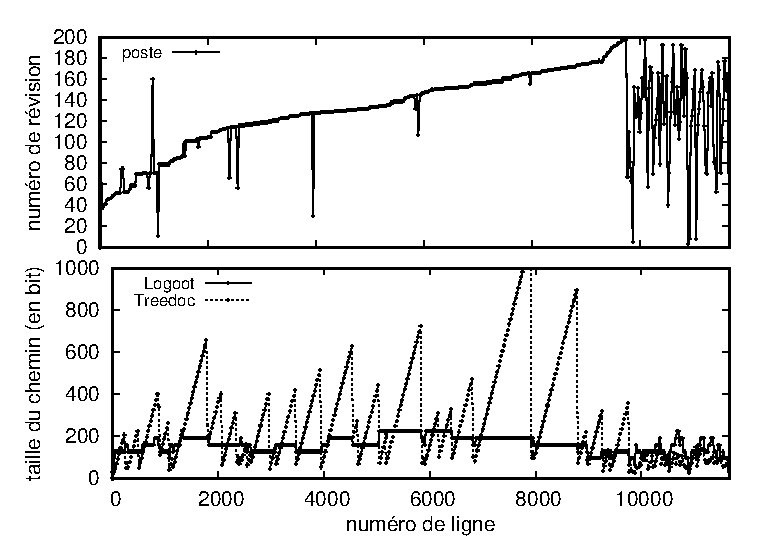
\includegraphics[width=0.8\textwidth]{img/lseq/motivationposte.eps}}
  \hspace{10pt}
  \subfloat[Document Wikipédia principalement édité au début]
  [\label{repl:img:motivationsB}Document Wikipédia de petite taille
  principalement édité au début.]
  {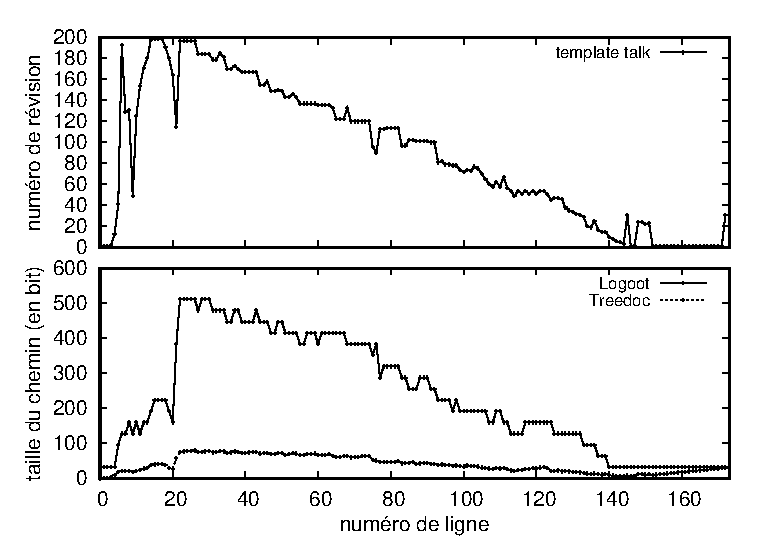
\includegraphics[width=0.8\textwidth]{img/lseq/motivationtemplatetalk.eps}}
  \caption[Taille du chemin alloué pour chaque ligne dans Wikipédia]
  {\label{repl:img:motivations} Taille du chemin alloué pour chaque ligne du
    document. L'axe des abscisses montre le numéro de la ligne concernée. L'axe
    des ordonnées de la partie haute de la figure montre l'âge de la
    ligne. L'axe des ordonnées de la partie basse de la figure montre la taille
    binaire du chemin alloué.}
\end{figure*}

L'encyclopédie Wikipédia~\cite{wikipedia} répertorie des millions d'articles
écrits collaborativement par sa communauté. Un utilisateur, enregistré ou non,
peut lire un article, et s'il le souhaite, en modifier le contenu. Lorsque ses
modifications sont achevées, il les soumet à Wikipédia. Deux issues possibles :
\begin{inparaenum}[(i)]
\item La contribution est acceptée et sera visible de tous ou
\item la contribution est rejetée car un autre utilisateur a effectué une
  modification en concurrence et l'a soumise en premier. Il faut alors réviser
  la version rejetée afin de l'adapter à la version la plus à jour avant de la
  soumettre à nouveau, si nécessaire.
\end{inparaenum}
Wikipédia garde l'historique des modifications apportées à tous les articles
depuis leur création. Nous sommes alors à même de rejouer les éditions --
nommées révision -- dans l'ordre où elles ont été effectuées. Toutefois, la
concurrence qui pourrait exister dans une édition en temps réelle est effacée
par le processus d'édition même. D'autre part, la granularité est fixée à la
ligne. En cela, les simulations sur corpus Wikipédia diffèrent légèrement de la
réalité.

\paragraph{Objectif :} Montrer que ni Logoot ni Treedoc ne parviennent pas à
fournir des identifiants dont la taille soit satisfaisante quel que soit le
document créé grâce à des traces réelles.

\paragraph{Description :} Logoot est configuré avec une base $2^{32}$. Treedoc
est configuré pour utiliser sa méthode originelle -- son autre heuristique
revenant plus ou moins à la stratégie de Logoot. Les documents considérés sont
des articles extraits de Wikipédia et rejoués sur 200 révisions. L'un des
articles atteint jusqu'à 10k lignes principalement ajoutées en fin
d'article\footnote{\scriptsize\url{https://fr.wikipedia.org/wiki/Liste_des_bureaux_de_poste_français_classés_par_oblitération_Petits_Chiffres}}. L'autre
article atteint seulement 200 lignes mais est principalement édité en
tête\footnote{\scriptsize\url{https://en.wikipedia.org/wiki/Template_talk:Did_you_know}}.

\paragraph{Résultat :} Les figures~\ref{repl:img:motivationsA}
et~\ref{repl:img:motivationsB} montrent la taille de l'identifiant associé à
chaque ligne. Nous observons que Treedoc possède des chemins qui augmentent très
vite quel que soit le type d'édition. Lorsque le nombre d'insertions successives
est très grand (cf. figure~\ref{repl:img:motivationsA}) les chemins atteignent
des tailles très élevée dépassant les 1k bits par chemin. Dans ce cas, Logoot se
comporte mieux. En revanche, dans le cadre de l'édition en tête, Logoot alloue
des chemins dont la taille augmente extrêmement rapidement. Pour recouvrer de
bonnes performances, l'exécution d'un protocole de relocalisation des chemins
devient nécessaire.

\paragraph{Explication :} Dans les deux types d'édition, Treedoc et Logoot
allouent des identifiants dont la complexité est linéaire. Ainsi, plus les
insertions se succèdent, plus l'arbre est déséquilibré, plus la taille du chemin
augmente. Cependant, comme l'arité des chemins Treedoc est binaire
($\mathcal{P}\in \mathbb{N}_{<2}.\mathbb{N}_{<2}\ldots\mathbb{N}_{<2}$), cela
lui permet de conserver des chemins plus petits que ceux de Logoot dans le cadre
du document édité en tête. D'un autre coté, Logoot a conçu sa stratégie pour
l'édition en fin. Dès lors, si le comportement suit cette hypothèse, les
identifiants grossissent par paliers. Linéairement certes, mais lentement. Dans
le cas contraire, les identifiants grimpent très rapidement (cela serait le cas
avec la seconde heuristique de Treedoc).

\subsubsection{Documents artificiels}


\begin{figure}
  \begin{center}
    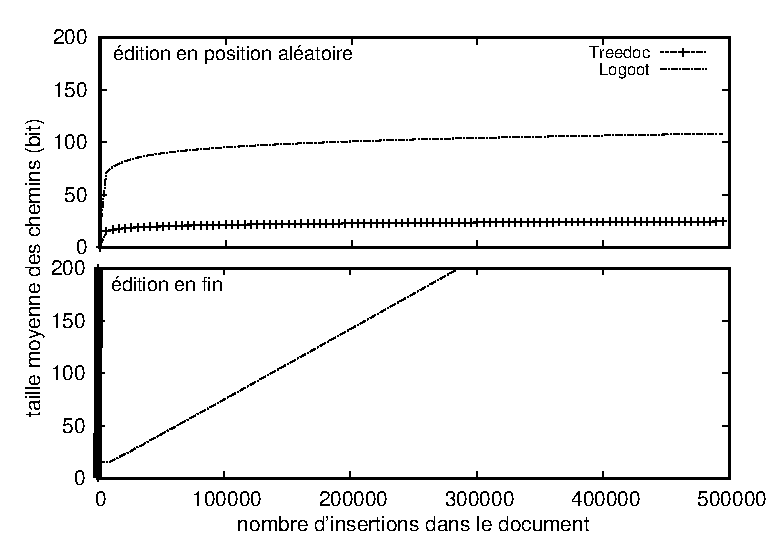
\includegraphics[width=0.8\textwidth]{img/lseq/motivationartificial.eps}
    \caption[Taille moyenne des chemins sur des documents artificiels]
    {\label{repl:img:motivationartificial}Taille moyenne des chemins
      allouées en fonction du nombre d'insertions successives dans le
      document. L'axe des abscisses montre le nombre d'insertions dans le
      documents. L'axe des ordonnées montre la taille moyenne de la
      représentation binaire des chemins alloués.}
  \end{center}
\end{figure}

\paragraph{Objectif :} Montrer la progression de la taille des identifiants
allouées par les fonctions d'allocation Logoot et Treedoc sur des documents
artificiels.

\paragraph{Description :} Deux types de documents artificiels sont créés. Tout
d'abord, un premier document est créé grâce à des insertions à des positions
aléatoires dans la séquence. Le second document est créé grâce à des insertions
successives en fin de document. La fonction d'allocation des chemins de Logoot
est spécifiquement conçue pour gérer ce dernier type d'édition. La taille
moyenne des chemins composant les identifiants est mesurée à chaque nouvelle
insertion. Le document atteint 500k caractères.

\paragraph{Résultat :} La figure~\ref{repl:img:motivationartificial} montre les
résultats de cette simulation. La partie du haut montre les résultats du
document édité à des positions aléatoires. La partie du bas montre les résultats
du document édité à la fin. Nous observons que l'édition à des positions
aléatoires entraîne une génération de chemins dont la taille est logarithmique,
que ce soit pour Logoot ou pour Treedoc. Treedoc est meilleur que Logoot dans ce
cas. Nous observons aussi que l'édition en fin est catastrophique pour Treedoc
(la courbe est superposée à l'axe des ordonnées). De son coté, Logoot alloue des
chemins dont la taille augmente moins rapidement. Malgré cela, la croissance
reste linéaire. À terme, l'exécution d'un protocole de relocalisation des
chemins devient nécessaire pour recouvrir de bonnes performances.

\paragraph{Explication :} Les fonctions d'allocations Logoot et Treedoc
utilisent une structure d'arbres pour allouer le chemin associé à chaque
caractère. Dans le cadre de l'édition aléatoire, l'arbre reste équilibré au
cours des insertions. Les branches les plus basses se remplissent au maximum de
leur capacité. Par conséquent, les identifiants alloués par Treedoc et Logoot
croissent logarithmiquement par rapport au nombre d'insertion. L'arité de
l'arbre de Treedoc étant inférieure à l'arité de l'arbre de Logoot, Treedoc
propose de meilleures performances. Dans le cadre de l'édition en fin, chaque
nouvelle insertion dans Treedoc ajoute un bit au chemin généré. La croissance
est linéaire comparée au nombre d'insertions dans la séquence et extrêmement
rapide. La fonction d'allocation de Logoot est conçue pour gérer ce type
d'édition. Une branche par niveau de l'arbre se trouve bien remplie
d'éléments. Toutefois, le nombre d'éléments accueillis par chaque branche reste
constant, d'où la croissance linéaire de la taille des chemins générés.



%%% Local Variables:
%%% mode: latex
%%% TeX-master: "../../paper"
%%% End:
